\documentclass{poly}
\usepackage{main}

\title{Fonctions exponentielles et logarithmiques}
\author{Terminale STMG}
\date{}

\begin{document}
\maketitle
\section{Fonction exponentielle}
\subsection{Définition de l'exponentielle de base $a$}
\begin{tcolorbox}
On représente ci-contre les valeurs de la suite géométrique $(u_n)_{n \in \N}$ définie par $u_n = a^n$, avec $a > 0$.
\end{tcolorbox}
\begin{center}
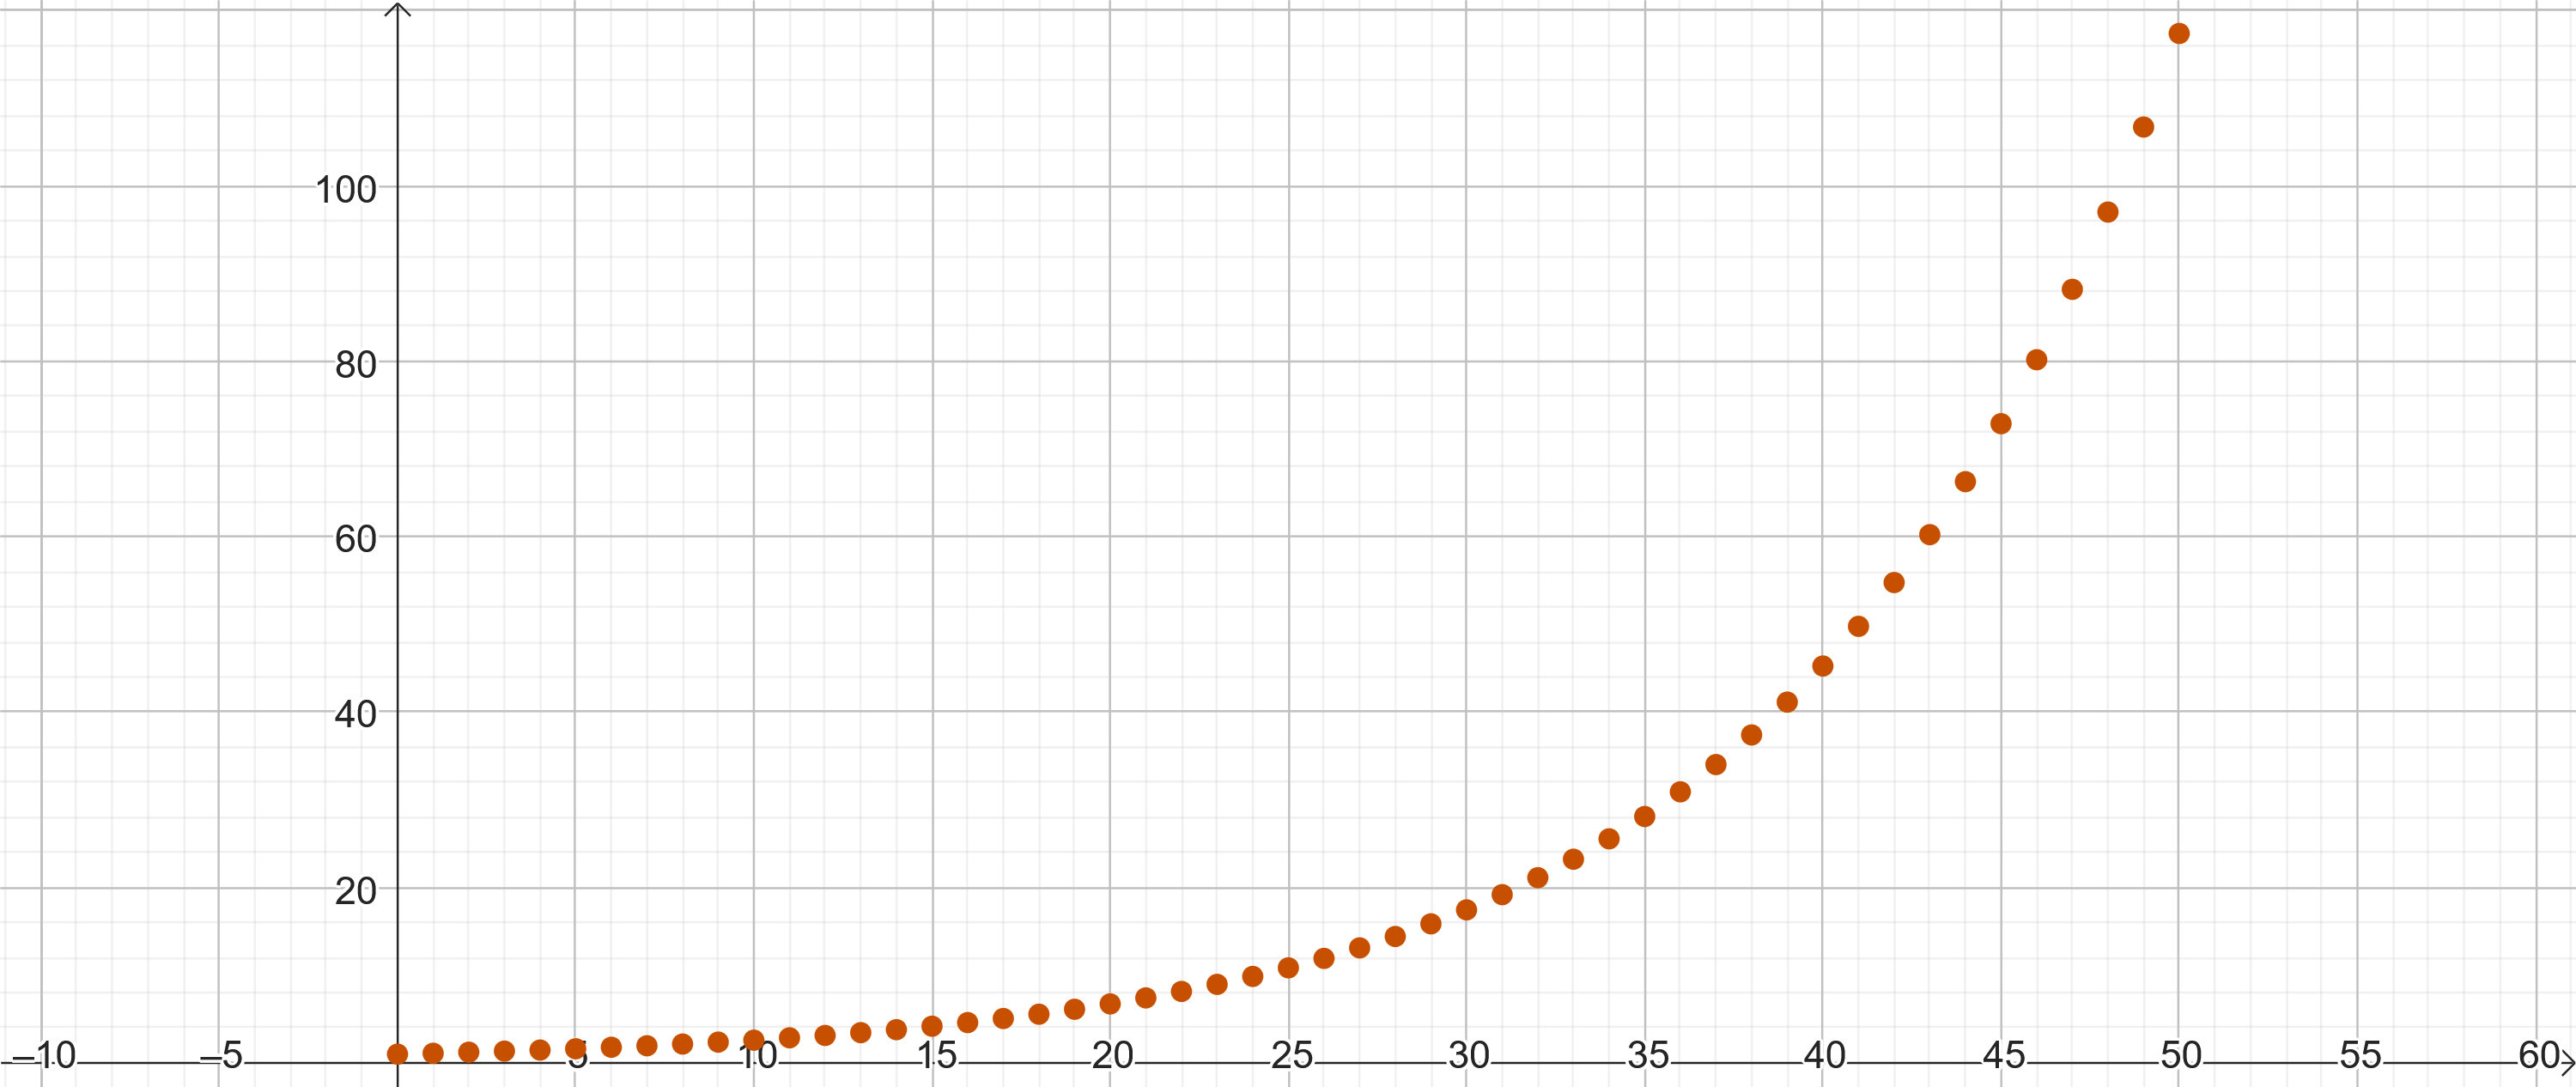
\includegraphics[width=\textwidth]{Suite_geometrique.png}
\end{center}
\begin{definition}
Le prolongement aux réels de la suite $u_n$ est appelée \textbf{fonction exponentielle de base $a$}. Pour tout $x$ réel, l'image de $x$ par cette fonction est notée $a^x$. En particulier, si $x < 0$, alors cette image est définie par:
\begin{equation*}
a^x = \dfrac{1}{a^{-x}}
\end{equation*}
\end{definition}
\begin{example}
À l'aide d'une calculatrice, donner la valeur des image de fonctions exponentielles suivantes :
\begin{alphaquestions}
\item $2^{3,5} = $
\item $10,2^{0,2} = $
\item $0,6^{-5,4} = $
\end{alphaquestions}
\end{example}

\subsection{Représentation graphique}
On représente ci-dessous la courbe représentative d'une fonction exponentielle de base $a$. Elle correspond au prolongement des points de coordonnées $(n;a^n)$.
\vspace*{0.5cm}
\begin{center}
\begin{minipage}{0.45\textwidth}
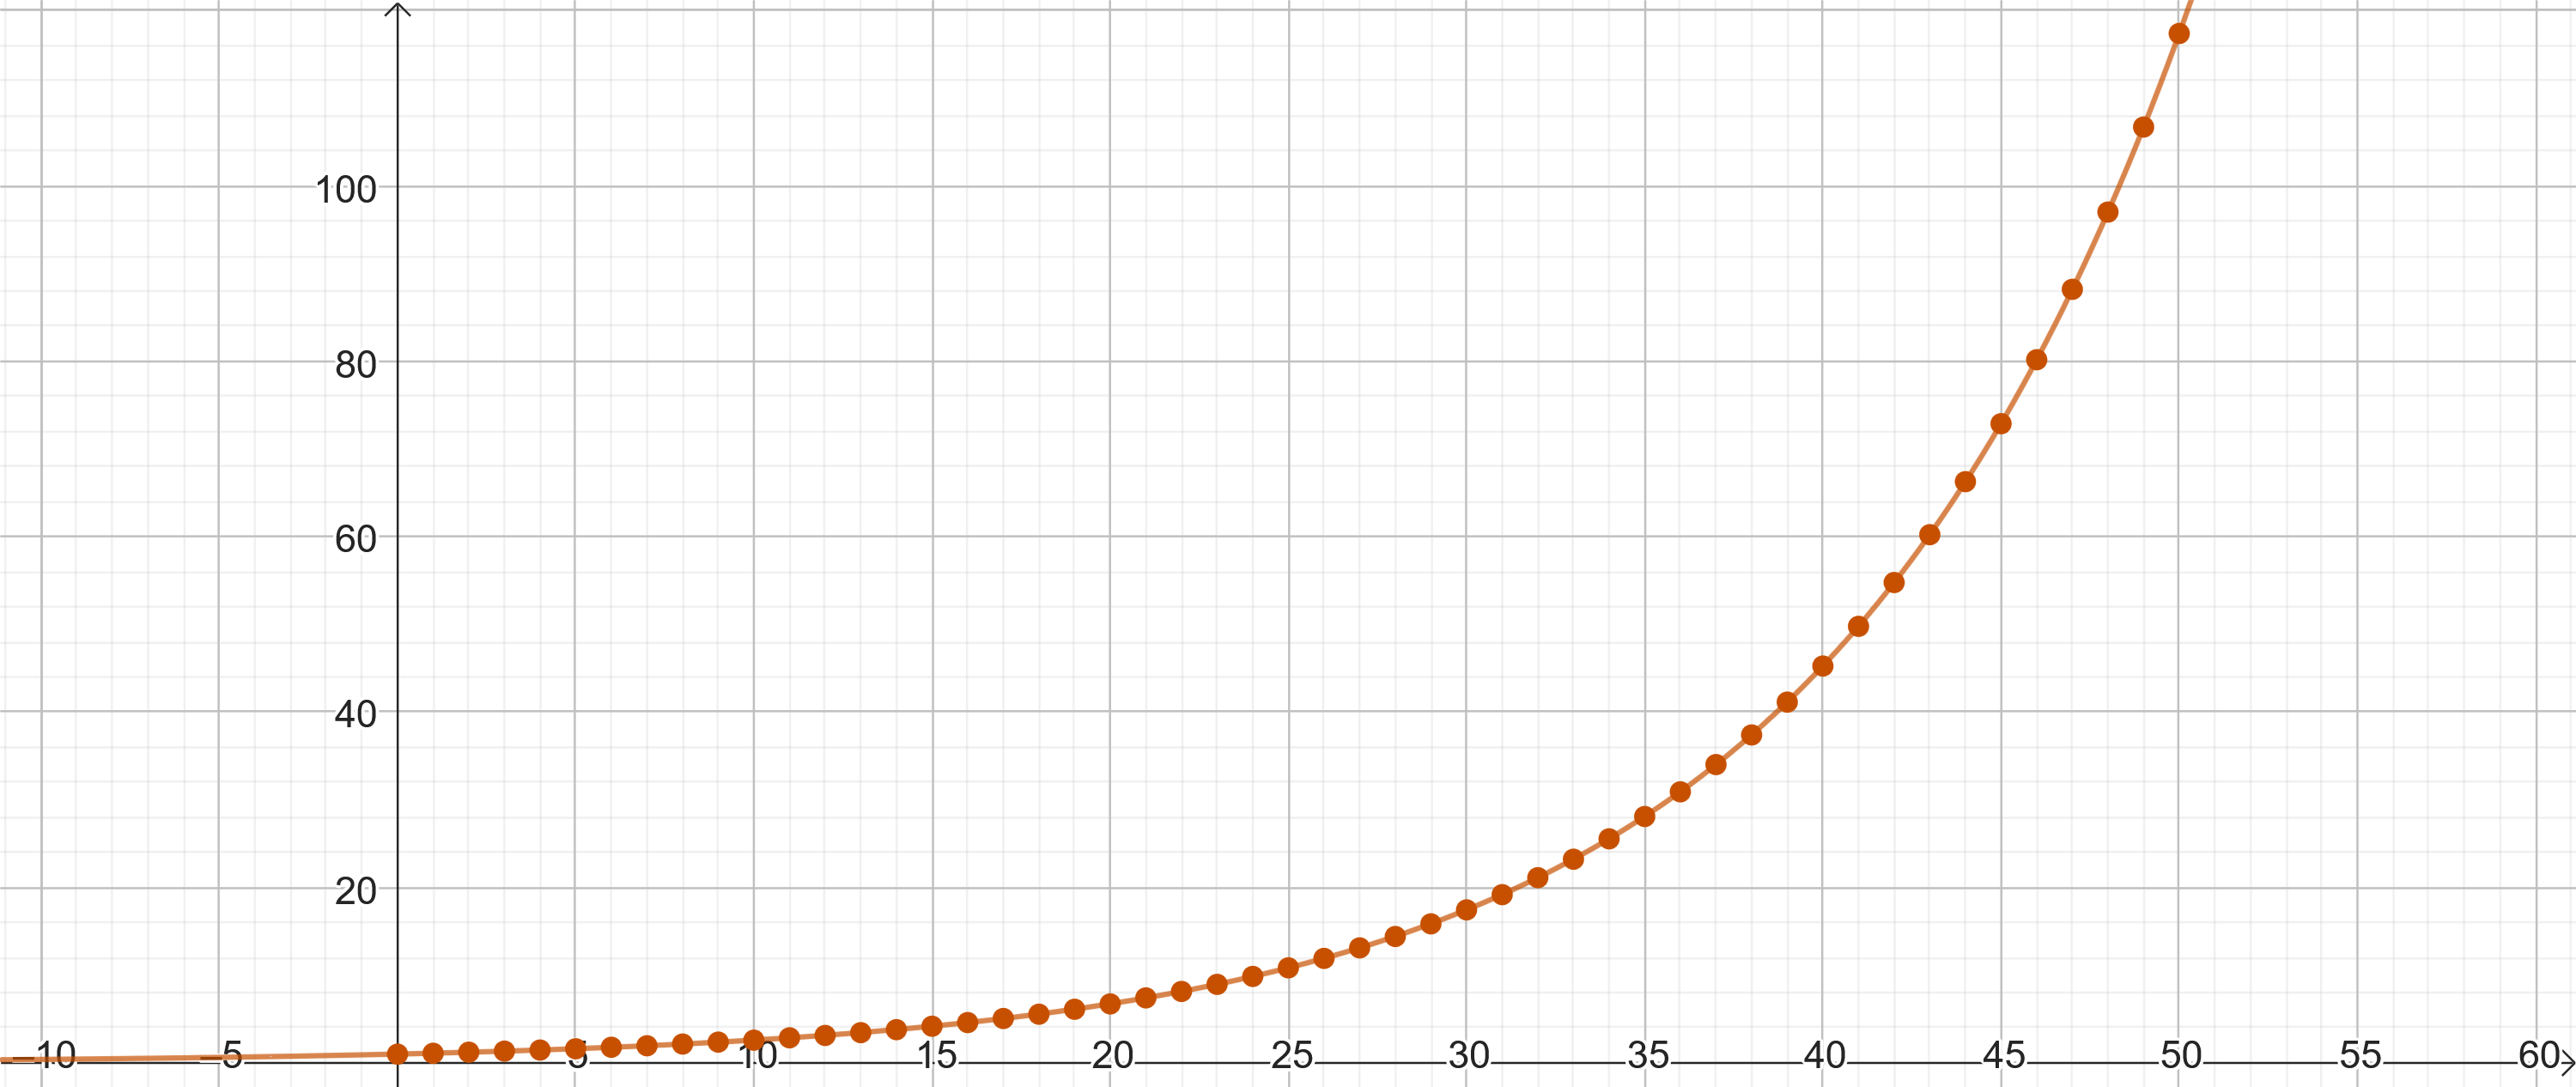
\includegraphics[width=\textwidth]{Fonction_exponentielle.png}
\end{minipage}
\begin{minipage}{0.45\textwidth}
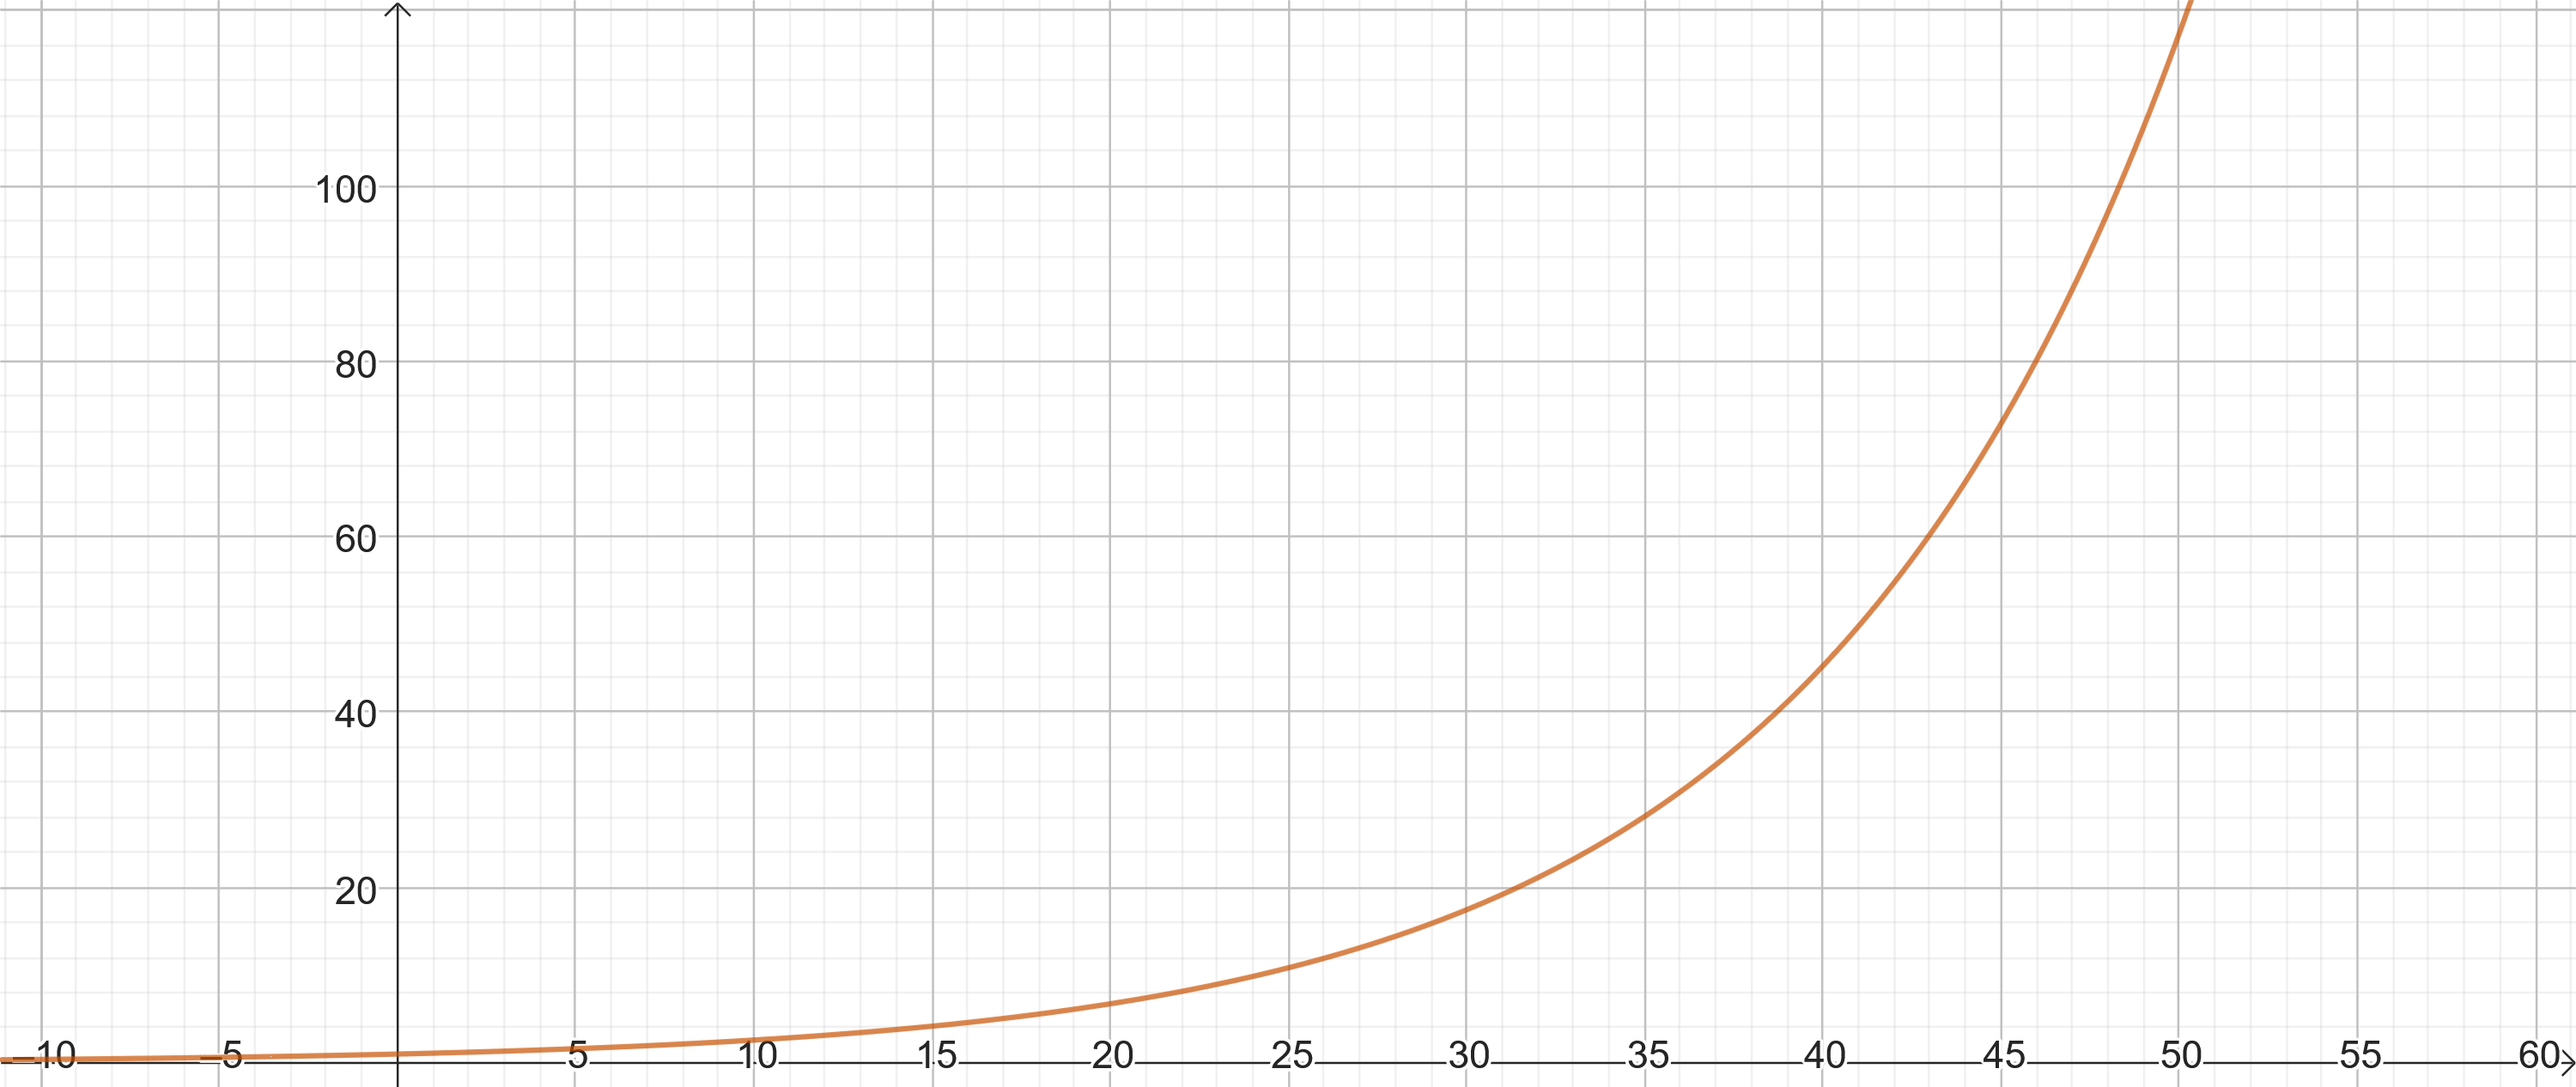
\includegraphics[width=\textwidth]{Fonction_exponentielle_2.png}
\end{minipage}
\end{center}
\subsection{Sens de variation}
\begin{proposition}
Soit $a > 0$ un nombre réel. Alors,
\begin{itemize}
\item La fonction exponentielle de base $a$ est strictement croissante si et seulement si $a > 1$. 
\item La fonction exponentielle de base $a$ est strictement décroissante si et seulement si $a < 1$. 
\item La fonction exponentielle de base $a$ est constante si et seulement si $a = 1$. 
\end{itemize}
\end{proposition}
\begin{center}
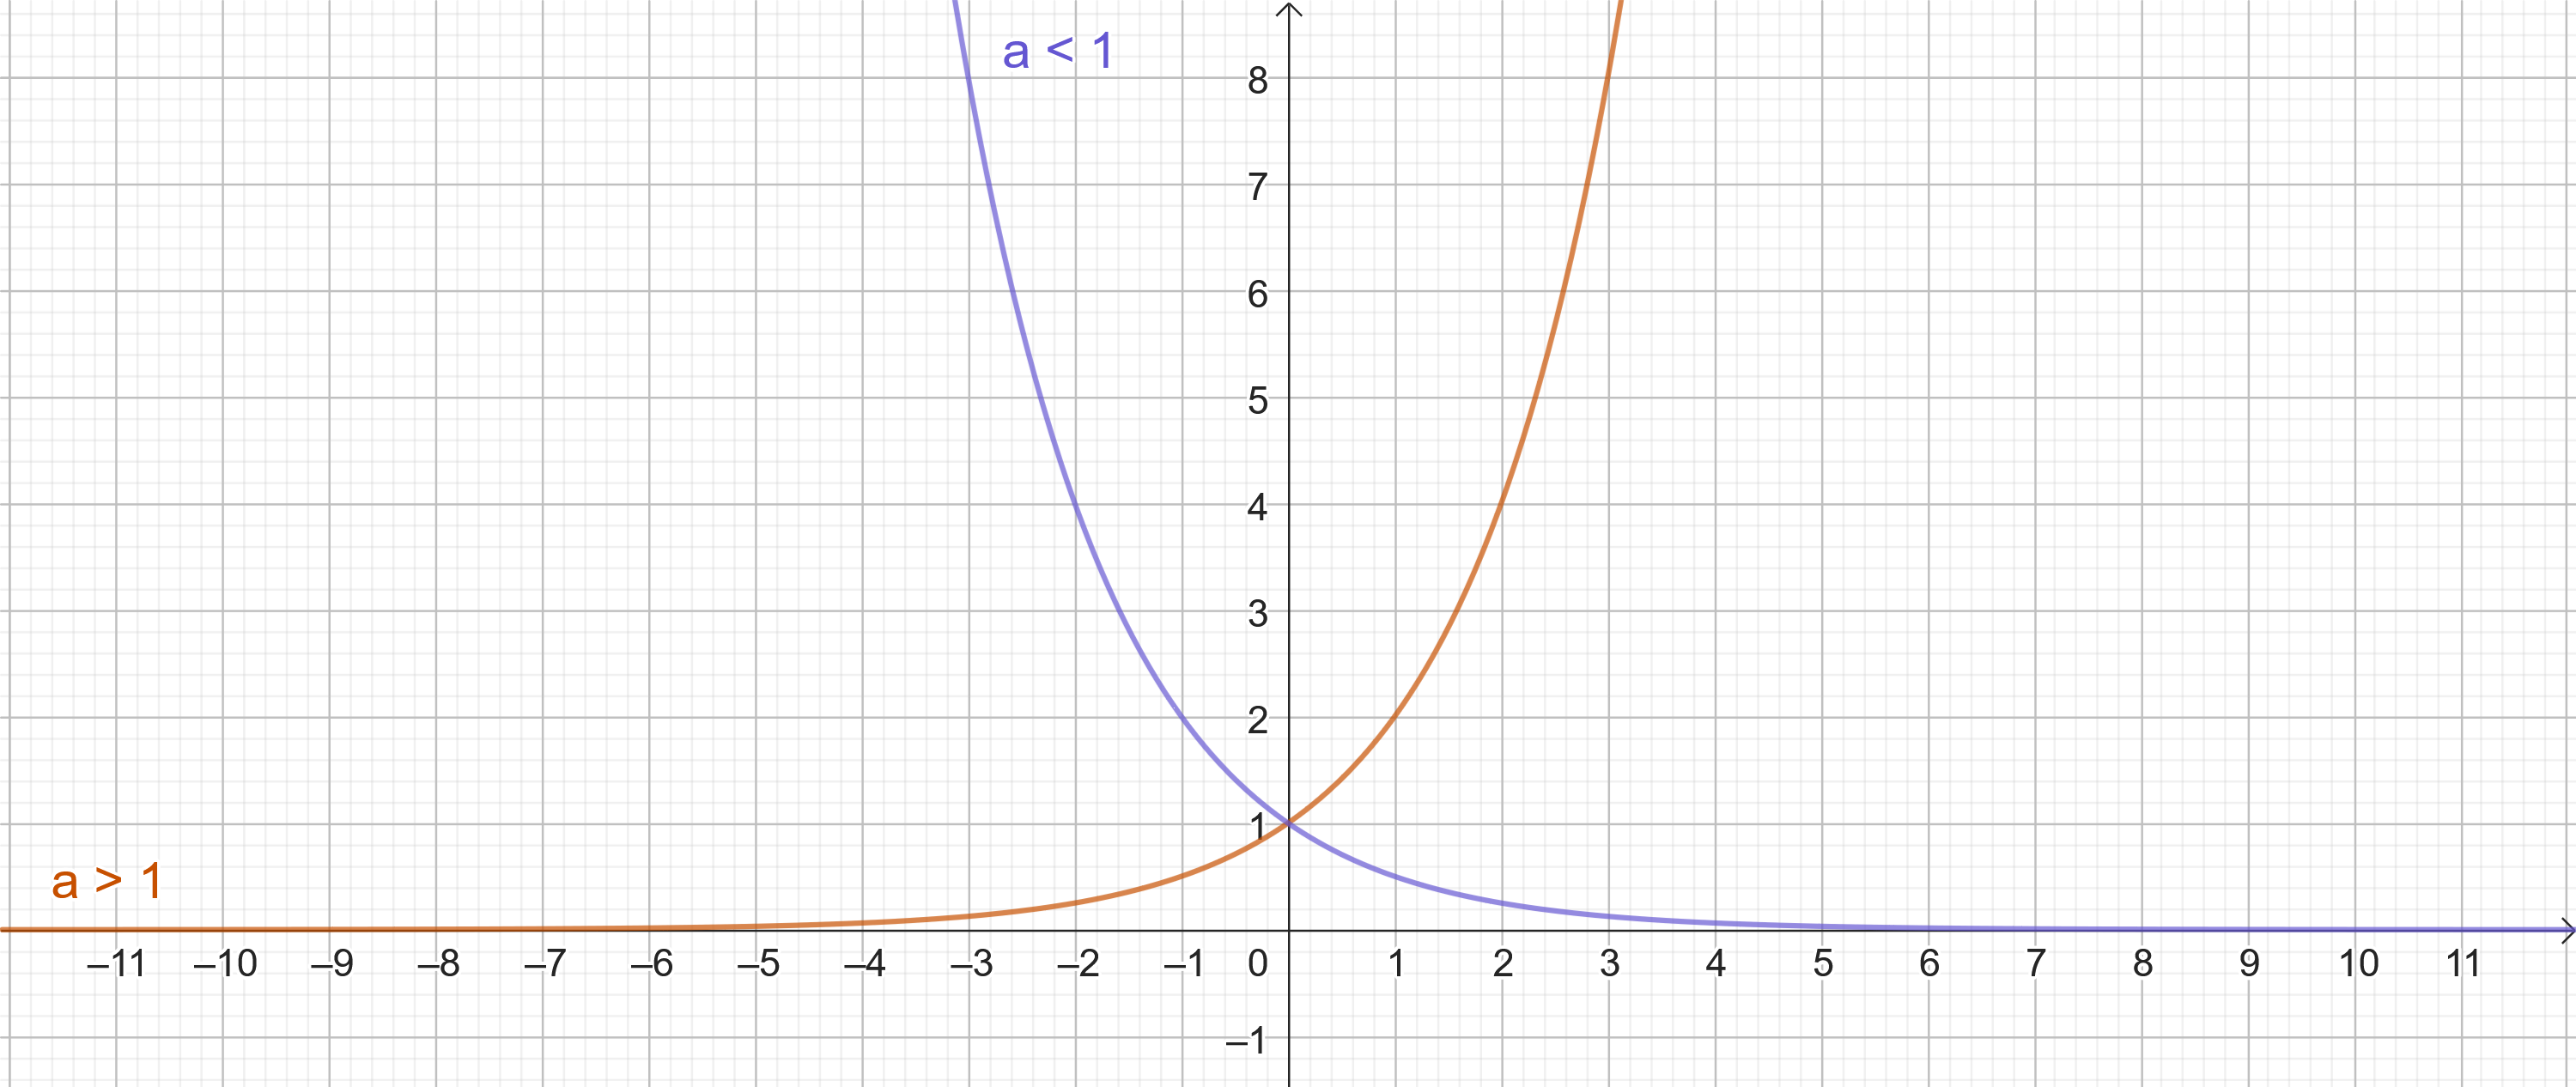
\includegraphics[width=\textwidth]{Variation_exponentielle.png}
\end{center}
\begin{example}
\hfill
\begin{alphaquestions}
\item Comparer $3,4^{12}$ et $3,4^{15}$ : 
\item Comparer $0,7^{3}$ et $0,7^{9}$ : 
\end{alphaquestions}
\end{example}
\begin{proposition}
Soit une fonction de la forme $f : x \mapsto k a^x$ avec $k$ un nombre réel et $a > 0$, alors le sens de variation de $f$ est donné grâce au tableau suivant.
\begin{center}
\begin{tabular}{|c|c|c|}
\hline
&$a > 1$&$a < 1$\\
\hline
$k > 0$& Croissante & Décroissante\\
\hline
$k < 0$& Décroissante & Croissante\\
\hline
\end{tabular}
\end{center}
\end{proposition}

\subsection{Propriétés algébrique de la fonction exponentielle}
\begin{proposition}
Soit $a$ un réel positif, ainsi que $x,y$ deux réels quelconques. Alors,
\begin{itemize}
\item $a^{x+y}=a^x \times a^y$
\item $a^{x \times y} = (a^x)^y$
\item $a^{x - y} = \dfrac{a^x}{a^y}$
\item $a^{-x} = \dfrac{1}{a^x}$
\item $a^{1/n} = \sqrt[n]{a}$
\item $a^0 = 1$
\end{itemize}
\end{proposition}
\begin{example}
Simplifier les expressions suivantes en une puissance de $2$ :
\begin{alphaquestions}
\begin{minipage}{0.45\textwidth}
\item $2^{15} \times 2^{12} = $ 
\item $2^{-7} =$  
\item $(2^{12})^{-5} =$ 
\end{minipage}
\hfill
\begin{minipage}{0.45\textwidth}
\item $\dfrac{2^{18}}{2^5} = $ 
\item $64^{4} =$  
\item $2^4 + 2^4 =$ 
\end{minipage}
\end{alphaquestions}
\end{example}
\subsection{Cas particulier : taux d'évolution moyen}
\begin{definition}
On suppose qu'une quantité évolue de $T\%$ en $n$ étapes. Alors, si le coefficient multiplicateur de $T$ est noté $CM$, on dit que le \textbf{taux d'évolution moyen} est donné par le taux d'évolution $t$ dont le coefficient multiplicateur $cm$ est donné par
\begin{equation*}
cm = CM^{1/n}
\end{equation*}

Cela correspond au taux d'évolution constant associé à une étape. 
\end{definition}
\begin{center}
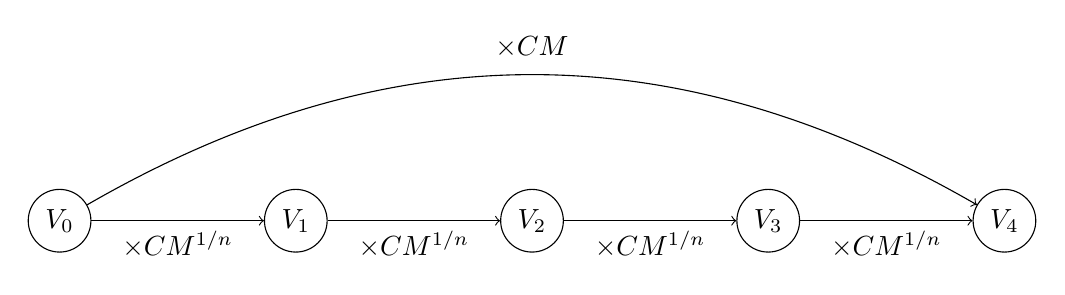
\begin{tikzpicture}
\node[draw,circle] (V0) at (0,0) {$V_0$};
\node[draw,circle] (V1) at (3,0) {$V_1$};
\node[draw,circle] (V2) at (6,0) {$V_2$};
\node[draw,circle] (V3) at (9,0) {$V_3$};
\node[draw,circle] (V4) at (12,0) {$V_4$};
\draw[->] (V0) -- (V1) node[midway,below] {$\times CM^{1/n}$};
\draw[->] (V1) -- (V2) node[midway,below] {$\times CM^{1/n}$};
\draw[->] (V2) -- (V3) node[midway,below] {$\times CM^{1/n}$};
\draw[->] (V3) -- (V4) node[midway,below] {$\times CM^{1/n}$};
\draw[->] (V0) to[bend left] (V4);
\draw (6,2.2) node {$\times CM$};
\end{tikzpicture}
\end{center}
\begin{example}
Le prix du loyer augmente de $54\%$ en quatre ans. Donner le taux d'évolution moyen de cette augmentation.

\begin{alphaquestions}
\item On calcule d'abord le coefficient multiplicateur de $+ 54\%$ : $CM = $ 
\item On calcule ensuite $cm = CM^{1/4} = $ 
\item On déduit le taux d'évolution moyen $t = cm - 1 =$ 
\end{alphaquestions}
\end{example}
\newpage
\section{Fonction logarithme décimal}
\subsection{Définition du logarithme décimal}
\begin{definition}
Soit $a$ un nombre réel \textbf{non nul positif}. L'équation $10^x = a$ admet une unique solution. Cette solution est notée $\log(a)$.
\end{definition}
\begin{example}
Donner les équations dont les nombres $\log(2)$; $\log(5)$ et $\log(\pi)$ sont solution.
\end{example}
\begin{definition}
La fonction $\log : x \mapsto \log(x)$ est nommée \textbf{fonction logarithme décimal}. Elle est définie sur $]0;+\infty[$.
\end{definition}
\subsection{Étude de la fonction}
\begin{center}
\begin{tikzpicture}
  
\begin{axis}[xmin=-1,xmax=10, enlargelimits, xtick distance = 1]
\addplot[domain=0.01:15] {ln(x)/ln(10)};
\end{axis}
\end{tikzpicture}
\end{center}
\begin{proposition}
La fonction $\log$ est strictement croissante sur $]0;+\infty[$.
\end{proposition}
\begin{proposition}
\begin{equation*}
\log(1)=0 \quad \log(10) = 1
\end{equation*}
\end{proposition}
\subsection{Propriétés algébriques}
\begin{proposition}
Soit $x; y$ deux réels strictement positifs.
\begin{equation*}
\begin{tblr}{}
\log(xy) = \log(x) + \log(y) & \log\left(\dfrac{x}{y}\right) = \log(x) - \log(y)\\
\log(x^n) = n \log(x) & \log\left(\dfrac{1}{x}\right) = - \log(x)
\end{tblr}
\end{equation*}
\end{proposition}
\newpage
\subsection{Résolution d'équations}
\begin{proposition}
Soient $x,y$ deux nombres réels strictement positifs. Alors:
\begin{itemize}
\item $\log(x) = \log(y)$ si et seulement si $x = y$
\item $\log(x) < \log(y)$ si et seulement si $x < y$
\end{itemize}
\end{proposition}
\begin{example}
Résoudre les équations et inéquations suivantes:
\begin{alphaquestions}
\item $\log(3x + 2) = \log(5)$
\item $\log(3x - 4) = \log(6x + 2)$
\item $\log(x^2) \leq \log(4)$
\item $\log(14x - 13) = 0$
\end{alphaquestions}
\end{example}
\begin{proposition}
Soient $a$ et $k$ deux nombres réels strictement positifs. Pour résoudre une équation de la forme $a^x = k$ ou une inéquation de la forme $a^x \leq k$, on \og passe au logarithme \fg.
\end{proposition}
\begin{example}
Soit l'inéquation $2^x \geq 5$. Alors,
\begin{equation*}
\begin{aligned}
2^x \geq 5 &\Leftrightarrow \log(2^x) \geq \log(5)\\
&\Leftrightarrow x\log(2) \geq \log(5)\\
&\Leftrightarrow x \geq \dfrac{\log(5)}{\log(2)}\\
\end{aligned}
\end{equation*}
(Le symbole d'inégalité ne change pas car $\log(2)$ est positif)
\end{example}
\end{document}